\documentclass[a4paper,fleqn,12pt]{cas-sc}

\usepackage[utf8]{inputenc}
\usepackage[T5,T1]{fontenc}
\DeclareTextFontCommand{\textvn}{\fontencoding{T5}\selectfont}

\usepackage[numbers,sort&compress]{natbib}
\usepackage{graphicx}
\usepackage{amsmath,amssymb,amsfonts,bm}
\usepackage{booktabs}
\usepackage{tabularx}
\usepackage{float}
\usepackage[section]{placeins}
\usepackage{hyperref}
\usepackage{tikz}
\usepackage{url}
\usepackage{multirow}
\usepackage{array}
\usepackage{microtype}
\microtypesetup{expansion=false}
\usepackage{makecell}
\usepackage{enumitem}

% Academic Hyperref Configuration
\hypersetup{
    colorlinks=true,
    linkcolor=cyan!80!black,
    citecolor=cyan!80!black,
    urlcolor=cyan!80!black
}

\newcommand{\orcidicon}[1]{\href{https://orcid.org/#1}{\texorpdfstring{%

\begin{tikzpicture}[baseline=-0.4ex]%
\definecolor{orcidgreen}{HTML}{A6CE39}%
\draw[fill=orcidgreen,draw=none] (0,0) circle (1.0ex);%
\node at (0,0) {\color{white}\fontsize{4}{4}\selectfont\sffamily\bfseries iD};%
\end{tikzpicture}%
}{}}}

\setcounter{topnumber}{4}
\setcounter{bottomnumber}{4}
\setcounter{totalnumber}{8}
\setcounter{dbltopnumber}{4}
\renewcommand{\topfraction}{0.95}
\renewcommand{\bottomfraction}{0.90}
\renewcommand{\textfraction}{0.05}
\renewcommand{\floatpagefraction}{0.75}

\ExplSyntaxOn
\cs_set:Npn \__reset_fig:
{
  \tl_set:Nx \l_fig_pos_tl { t }
  \tl_set:Nx \l_fig_cols_tl { 1 }
  \tl_set:Nn \l_fig_align_tl { \centering }
  \skip_set:Nn \l_fig_abovecap_skip { 6pt }
  \skip_set:Nn \l_fig_belowcap_skip { 6pt }
  \skip_set:Nn \l_fig_abovefig_skip { 6pt }
  \skip_set:Nn \l_fig_belowfig_skip { 6pt }
}
\tl_set:Nn \l_fig_align_tl { \centering }

\cs_set:Npn \__first_footerline: {}
\cs_set:Npn \__first_foot: 
{%
  \noindent\begin{minipage}[b]{\linewidth}%
    \setlength{\parindent}{0pt}%
    \noindent\rule{0.32\linewidth}{.4pt}\par\vspace{3pt}%
    \noindent\footnotesize\rmfamily%
    \textsuperscript{*}Corresponding author.\par\vspace{1pt}%
    \noindent\hspace*{1.1em}\textit{E-mail addresses:}~\href{mailto:khanhnt@ptit.edu.vn}{khanhnt@ptit.edu.vn}~(K.~Nguyen-Trong),~\href{mailto:anhlv.b23kh002@stu.ptit.edu.vn}{anhlv.b23kh002@stu.ptit.edu.vn}~(V.-A.~Le)%
  \end{minipage}%
}
\cs_set:Npn \__cas_foot: 
{%
  \noindent\begin{minipage}[t]{\linewidth}%
    \setlength{\parindent}{0pt}%
    \noindent\rule{\linewidth}{.2pt}\par\vspace{2pt}%
    \sffamily\small%
    \__first_footerline:%
    \hfill Page~\thepage {}~of~ \lastpage%
  \end{minipage}%
}
\ExplSyntaxOff
\let\printorcid\relax

\makeatletter
\setlength{\@fptop}{0pt}
\setlength{\@fpbot}{0pt plus 1fil}
\setlength{\@fpsep}{10pt plus 2fil}
\let\printFirstPageNotes\relax
\makeatother

\hyphenation{Afzelia Guibourtia Pterocarpus Dalbergia Sindora cochinchinensis melanoxylon pachyloba quanzensis arnoldiana coleosperma}

\begin{document}

\let\WriteBookmarks\relax

\shorttitle{IC4SDMacroWood: Benchmark Dataset for Timber Classification and Metric Learning}
\shortauthors{V.-A. Le and K. Nguyen-Trong}

\title [mode = title]{IC4SDMacroWood: A Forensic-Grade Macroscopic Timber Image Dataset with Fine-Grained Classification and Metric Representation Learning Benchmarks}

\author[1]{Viet-Anh Le \orcidicon{0009-0003-5748-0439}}
\author[1]{Khanh Nguyen-Trong \orcidicon{0000-0001-5175-8805}\cormark[1]}

\address[1]{Intelligent Computing for Sustainable Development Laboratory (IC4SD), Posts and Telecommunications Institute of Technology (PTIT), Hanoi, Vietnam}

\cortext[1]{Corresponding author. \textit{E-mail addresses:} \href{mailto:khanhnt@ptit.edu.vn}{khanhnt@ptit.edu.vn} (K. Nguyen-Trong), \href{mailto:anhlv.b23kh002@stu.ptit.edu.vn}{anhlv.b23kh002@stu.ptit.edu.vn} (V.-A. Le)}

\begin{abstract}
Automated timber species verification via macroscopic cross-sectional imaging provides a rapid, non-destructive screening capability vital for combating illegal logging, ensuring timber supply-chain traceability, and enforcing international trade controls under CITES Appendix~II. However, deploying reliable computer vision systems in this domain is severely challenged by fine-grained anatomical resemblances among congeneric sister taxa, deceptive commercial counterfeiting across phylogenetic clades, and natural collection imbalance. To address these operational demands, we present \textbf{IC4SDMacroWood}, an authenticated, forensic-grade image benchmark comprising exactly \textbf{7,278 standardized macroscopic cross-sectional captures} ($224 \times 224$ pixels at $50\times$ optical magnification, spatial resolution of $12\,\mu\text{m}$) spanning \textbf{19 commercial tropical hardwood species} from 6 botanical genera within the legume family \textbf{Fabaceae}. The benchmark encompasses 9 taxa strictly regulated under CITES Appendix~II and 4 high-value timber species endemic to Vietnam (\textit{Dalbergia cochinchinensis}, \textit{D.~tonkinensis}, \textit{Sindora cochinchinensis}, and \textit{S.~tonkinensis}). All wood specimens were surfaced, polished, cleaned, and imaged under calibrated diffuse LED illumination, with image quality audited through objective Laplacian focus filtering and bitwise SHA-256 cryptographic checksums. To ensure realistic, unbiased generalization, the repository is partitioned under a strict specimen-disjoint scheme ($N_{\text{train}} = 4,960$, $N_{\text{val}} = 1,253$, and $N_{\text{test}} = 1,065$), guaranteeing zero physical specimen leakage across splits while preserving 100\% species coverage. Alongside the curated image repository and structured metadata, we establish dual empirical baselines using the modern ConvNeXt-Tiny architecture: (i) a supervised fine-grained classification model optimized via Multiclass Focal Loss, attaining $94.67\%$ overall accuracy and an $88.02\%$ macro-averaged F1-score across all 19 taxa, and (ii) a deep metric representation learning framework via Semi-Hard Triplet Loss, which contracts the intra-to-inter class Euclidean distance ratio from $0.6845$ down to $0.2810$, elevates the Silhouette score to $0.5485$, and achieves $91.80\%$ Recall@1 nearest-neighbor retrieval. Grad-CAM visual heatmaps confirm that metric supervision guides network attention directly to authentic diagnostic anatomical markers—specifically open vessel lumens and concentric axial parenchyma bands. IC4SDMacroWood provides an open, forensic-grade testbed for machine learning benchmarks and automated wood anatomy.
\end{abstract}

\begin{keywords}
Macroscopic wood anatomy \sep Fabaceae tropical hardwoods \sep Timber forensics \sep CITES Appendix~II trade monitoring \sep Fine-grained image classification \sep Deep metric representation learning \sep ConvNeXt-Tiny
\end{keywords}

\maketitle

\section*{Specifications Table}

\noindent
\small
\setlength{\tabcolsep}{5pt}
\renewcommand{\arraystretch}{1.12}
\begin{tabularx}{\linewidth}{@{} l X @{}}
\toprule
\textbf{Subject} & Computer Science; Forestry and Wood Science \\
\midrule
\textbf{Specific subject area} & Computer Vision, Macroscopic Timber Identification, Deep Metric Representation Learning, Forest Products Forensics, CITES Trade Compliance \\
\midrule
\textbf{Type of data} & Standardized macroscopic cross-sectional images ($50\times$ magnification, $224 \times 224$ px, RGB JPEG), deep feature embeddings ($\mathbb{R}^{768}$), structured metadata tables (CSV), and taxonomic mappings (JSON) \\
\midrule
\textbf{How the data were acquired} & Transverse end-grain surfaces surfaced orthogonally on an industrial sliding table saw, progressively polished across four grit gradations (P120--P600), cleaned with dry compressed-air jets, and captured at $50\times$ optical magnification ($12\,\mu\text{m}$ spatial resolution) under calibrated daylight-balanced ($5600\,\text{K}$) diffuse LED ring illumination \\
\midrule
\textbf{Data format} & Standardized $224 \times 224$ px RGB images (JPEG), deep feature embeddings (\texttt{.npy}), structured metadata tables (CSV), and label mappings (JSON) \\
\midrule
\textbf{Parameters for data collection} & Transverse wood sections; orthogonal end-grain surfacing; progressive silicon-carbide grit polishing; compressed-air vascular lumen de-dusting; uniform diffuse LED lighting at $50\times$ optical magnification \\
\midrule
\textbf{Description of data collection} & Curated from institutional timber collections supported by the Research Institute of Forest Industry (RIFI), Vietnamese Academy of Forest Sciences (VAFS), and collaborative activities associated with the GIZ-implemented FLEGT VPA project in Vietnam. The benchmark encompasses 19 commercially significant hardwood species across 6 botanical genera in the family Fabaceae, totaling exactly 7,278 standardized macroscopic cross-sectional captures partitioned under a strict specimen-disjoint allocation protocol ($N_{\text{train}} = 4,960$, $N_{\text{val}} = 1,253$, and $N_{\text{test}} = 1,065$) \\
\midrule
\textbf{Data source location} & \textbf{Institution:} Research Institute of Forest Industry (RIFI), Vietnamese Academy of Forest Sciences (VAFS), and Posts and Telecommunications Institute of Technology (PTIT), Hanoi, Vietnam \newline
\textbf{Repository:} Zenodo Scientific Archive \\
\midrule
\textbf{Data accessibility} & \textbf{Repository:} Zenodo Scientific Archive \newline
\textbf{DOI:} \href{https://doi.org/10.5281/zenodo.14892180}{10.5281/zenodo.14892180} \newline
\textbf{Code \& Manifests:} \url{https://github.com/vietanhlee/S3_paper} \\
\bottomrule
\end{tabularx}

\vspace{0.8em}

\section{Value of the Data}
\label{sec:value}

\begin{itemize}[leftmargin=*,itemsep=3pt,topsep=2pt]
    \item \textbf{Authoritative Reference for CITES Regulation and Endemic Taxa}: IC4SDMacroWood delivers an open, authenticated repository of 7,278 standardized macroscopic cross-sectional captures across 19 commercially significant tropical hardwood species in the family Fabaceae. Incorporating 9 taxa strictly regulated under CITES Appendix~II (notably within \textit{Afzelia} and \textit{Dalbergia}) and 4 high-value timber species endemic to Vietnam, the dataset serves as an authoritative forensic reference for border-control customs inspections and international wood trade surveillance.
    \item \textbf{Dual Empirical Benchmarking Testbed}: Beyond passive image curation, this benchmark supplies reproducible, standardized baselines for both supervised fine-grained classification under natural class imbalance (ConvNeXt-Tiny with Focal Loss) and deep metric representation learning (Semi-Hard Triplet Loss), providing a multi-dimensional comparative framework across all 19 taxa for future algorithm development.
    \item \textbf{Strict Specimen-Disjoint Partition Integrity}: To ensure realistic and leakage-free evaluation, all 7,278 images are partitioned strictly across physical wood blocks (Specimen-Disjoint: $N_{\text{train}} = 4,960$, $N_{\text{val}} = 1,253$, $N_{\text{test}} = 1,065$). This protocol guarantees that captures from identical wood samples never cross partition boundaries ($\text{SLR} = 0.0\%$) while maintaining a 100\% Class Coverage Rate across all 19 taxa.
    \item \textbf{Forensic Metadata and Optical Quality Assurance}: Every capture is cataloged with granular provenance metadata, physical specimen group identifiers (\texttt{specimen\_id}), objective focus sharpness scores ($\sigma^2_{\text{Laplacian}}$), and bitwise SHA-256 cryptographic checksums, guaranteeing complete transparency, auditability, and data integrity.
    \item \textbf{Pre-Extracted Deep Feature Representations}: The repository provides pre-computed, $L_2$-normalized 768-dimensional feature vectors extracted from ConvNeXt-Tiny, allowing researchers to explore clustering, metric learning, and nearest-neighbor retrieval without extensive computational or GPU infrastructure.
\end{itemize}

\section{Background}
\label{sec:background}

Illegal logging and transnational timber contraband account for an estimated US\$50--152 billion in illicit economic activity annually~\cite{dormontt2015,cites}, precipitating tropical deforestation, biodiversity collapse, and substantial fiscal revenue losses in timber-producing nations. In Southeast Asia and equatorial Africa, selective harvesting has driven commercially prized timber species—most notably endangered rosewoods (\textit{Dalbergia} spp.) and padauks (\textit{Pterocarpus} spp.)—to the brink of commercial extinction. In response, rigorous international trade controls have been established under CITES Appendix~II~\cite{cites}. Operationalizing these protections in field environments, however, necessitates rapid, non-destructive, and accurate timber authentication at border customs checkpoints and transit hubs~\cite{wiedenhoeft2011}.

While conventional microtome sectioning and histological light microscopy represents the traditional anatomical gold standard, it demands specialized histology laboratories, delicate physical sectioning, and several days of expert diagnostic review. Consequently, automated macroscopic wood identification using computer vision on transverse (end-grain) surfaces has emerged as the premier candidate for field-deployable screening~\cite{woodreview,ravindran2020,ravindran2022}.

Nevertheless, automated macroscopic timber identification confronts three profound computer vision challenges:
\begin{enumerate}[leftmargin=*,itemsep=2pt,topsep=2pt]
    \item \textbf{Intra-Genus Morphological Congruence}: Closely related species within the same botanical genus exhibit nearly identical cellular topographies on transverse cross-sections~\cite{liu2025,song2025}. For instance, \textit{Dalbergia cochinchinensis} and \textit{Dalbergia oliveri} both possess diffuse-porous solitary vessel distributions, overlapping pore diameters ($120$--$220\,\mu\text{m}$), and undulating concentric bands of axial parenchyma.
    \item \textbf{Inter-Genus Convergence and Commercial Counterfeiting}: Convergent anatomical evolution routinely produces matching macroscopic surface textures across divergent botanical genera~\cite{rosadasilva2022}. In commercial timber markets, non-CITES padauks (\textit{Pterocarpus macrocarpus} and \textit{P.~soyauxii}) are frequently substituted for endangered CITES-listed rosewoods (\textit{Dalbergia} spp.) due to overlapping reddish-brown heartwood coloration and tangential parenchyma patterns.
    \item \textbf{Natural Collection Imbalance}: Real-world forestry collection distributions inherently exhibit skewed specimen availability, ranging from 219 captures in scarce minority taxa (\textit{Afzelia pachyloba}) to 590 captures in abundantly traded taxa (\textit{Pterocarpus soyauxii}).
\end{enumerate}
The IC4SDMacroWood benchmark was curated to provide a standardized, leakage-controlled foundation for evaluating supervised classification and deep metric learning models under these demanding real-world conditions.

\section{Data Description}
\label{sec:description}

\subsection{Taxonomic Composition and Inventory}

The IC4SDMacroWood repository encompasses \textbf{19 commercially significant tropical hardwood species} spanning \textbf{6 botanical genera} within the legume family \textbf{Fabaceae} (Leguminosae), aggregating exactly \textbf{7,278 standardized macroscopic cross-sectional captures}. Curated from institutional timber reference archives at the Intelligent Computing for Sustainable Development Laboratory (IC4SD), PTIT, Hanoi, Vietnam, in collaboration with accredited forestry taxonomists, all 7,278 images possess verified species-level ground truth anchored to traceable physical wood specimens.

\begin{table}[pos=htbp]
\centering
\small
\setlength{\tabcolsep}{4.5pt}
\renewcommand{\arraystretch}{1.18}
\caption{Taxonomic inventory of the 19 tropical hardwood species in the IC4SDMacroWood benchmark, detailing genus, scientific binomial, native Vietnamese vernacular names, international trade names, CITES conservation status, and image counts.}
\label{tab:taxonomic_inventory}
\resizebox{\textwidth}{!}{%
\begin{tabular}{rlllllc}
\toprule
\textbf{\#} & \textbf{Botanical Genus} & \textbf{Scientific Binomial} & \textbf{Vietnamese Vernacular} & \textbf{Trade / Common Name} & \textbf{CITES Status} & \textbf{Total Images} \\
\midrule
1 & \textit{Afzelia} & \textit{A. africana} & \textvn{Gõ Douse (Gõ Doussié)} & African Doussié & CITES App.~II & 368 \\
2 & \textit{Afzelia} & \textit{A. bella} & \textvn{Papao-Nua / Gỗ Gõ} & Bella Doussié & CITES App.~II & 400 \\
3 & \textit{Afzelia} & \textit{A. pachyloba} & \textvn{Gõ Pachy} & White Doussié & CITES App.~II (Minority) & 219 \\
4 & \textit{Afzelia} & \textit{A. quanzensis} & \textvn{Gõ Quanzensis} & Pod Mahogany & CITES App.~II & 471 \\
\midrule
5 & \textit{Dalbergia} & \textit{D. cochinchinensis} & \textvn{Trắc (Rosewood)} & Siam Rosewood & CITES App.~II (Endemic VN) & 354 \\
6 & \textit{Dalbergia} & \textit{D. melanoxylon} & \textvn{Trắc châu Phi} & African Blackwood & CITES App.~II & 291 \\
7 & \textit{Dalbergia} & \textit{D. oliveri} & \textvn{Cẩm lai (Burmese Rosewood)} & Burmese Rosewood & CITES App.~II & 419 \\
8 & \textit{Dalbergia} & \textit{D. rimosa} & \textvn{Trắc dây} & Rimose Rosewood & Non-CITES & 300 \\
9 & \textit{Dalbergia} & \textit{D. tonkinensis} & \textvn{Sưa} & Vietnamese Rosewood & CITES App.~II (Endemic VN) & 325 \\
\midrule
10 & \textit{Guibourtia} & \textit{G. arnoldiana} & \textvn{Gỗ Muntenye} & Mutenye / Benge & Non-CITES & 323 \\
11 & \textit{Guibourtia} & \textit{G. coleosperma} & \textvn{Mussivi / Hương đá} & Rhodesian Copalwood & Non-CITES & 467 \\
12 & \textit{Guibourtia} & \textit{G. ehie} & \textvn{Hyedua} & Ovangkol / Shedua & Non-CITES & 400 \\
\midrule
13 & \textit{Peltogyne} & \textit{P. pubescens} & \textvn{Hương tím nam mỹ} & Purpleheart & Non-CITES & 371 \\
\midrule
14 & \textit{Pterocarpus} & \textit{P. erinaceus} & \textvn{Hương vân tây phi} & African Barwood / Kosso & CITES App.~II & 336 \\
15 & \textit{Pterocarpus} & \textit{P. indicus} & \textvn{Hương mắt chim} & Narra / Amboyna & Non-CITES & 312 \\
16 & \textit{Pterocarpus} & \textit{P. macrocarpus} & \textvn{Hương quả to} & Burma Padauk & Non-CITES & 550 \\
17 & \textit{Pterocarpus} & \textit{P. soyauxii} & \textvn{Padouk / Hương padouk} & African Padauk & Non-CITES & 590 \\
\midrule
18 & \textit{Sindora} & \textit{S. cochinchinensis} & \textvn{Gụ} & Sindora / Sepetir & Non-CITES (Endemic VN) & 454 \\
19 & \textit{Sindora} & \textit{S. tonkinensis} & \textvn{Gụ lau} & Tonkin Sepetir & Non-CITES (Endemic VN) & 328 \\
\midrule
\multicolumn{2}{l}{\textbf{Total Benchmark}} & \multicolumn{3}{l}{\textbf{19 Botanical Species (6 Genera, 9 CITES App.~II, 4 VN Endemics)}} & \textbf{Total Images} & \textbf{7,278} \\
\bottomrule
\end{tabular}%
}
\end{table}

Table~\ref{tab:taxonomic_inventory} details the taxonomic breakdown of the 19 species, providing scientific nomenclature, native Vietnamese vernacular terms, international trade designations, CITES conservation listings, and total image volumes.

\subsection{Repository Architecture and Metadata Schema}

The dataset package is organized systematically to facilitate seamless integration into machine learning pipelines. Table~\ref{tab:repo_contents} outlines the functional directory architecture, and Table~\ref{tab:metadata_fields} defines the structured metadata attributes cataloged in \texttt{metadata.csv}.

\begin{table}[pos=htbp]
\centering
\small
\setlength{\tabcolsep}{4pt}
\renewcommand{\arraystretch}{1.12}
\caption{Systematic directory layout and functional contents of the IC4SDMacroWood release package.}
\label{tab:repo_contents}
\begin{tabularx}{\linewidth}{@{} r l X @{}}
\toprule
\textbf{\#} & \textbf{File / Folder Path} & \textbf{Content Description and Functionality} \\
\midrule
1 & \texttt{images/} & 7,278 standardized $224 \times 224$ px macroscopic RGB images ($50\times$ magnification) organized by taxon. \\
2 & \texttt{metadata/metadata.csv} & Comprehensive master metadata table with image paths, taxonomic labels, specimen IDs, and QC scores. \\
3 & \texttt{metadata/label\_map.json} & Structured JSON mapping between integer class indices, scientific binomials, and vernacular names. \\
4 & \texttt{metadata/release\_manifest.csv} & Release manifest containing SHA-256 cryptographic hashes and byte sizes for integrity auditing. \\
5 & \texttt{splits/split\_canonical.csv} & Specimen-disjoint partition manifest ($N_{\text{train}} = 4,960$, $N_{\text{val}} = 1,253$, $N_{\text{test}} = 1,065$). \\
6 & \texttt{embeddings/convnext\_tiny.npy} & Pre-computed, $L_2$-normalized 768-dimensional feature vectors extracted via ConvNeXt-Tiny. \\
7 & \texttt{baseline\_outputs/} & Training logs, evaluation metrics, and figure artifacts for baseline reproducibility. \\
8 & \texttt{README.md}, \texttt{LICENSE} & Comprehensive documentation and Creative Commons Attribution 4.0 International license. \\
\bottomrule
\end{tabularx}
\end{table}

\begin{table}[pos=htbp]
\centering
\small
\setlength{\tabcolsep}{4pt}
\renewcommand{\arraystretch}{1.12}
\caption{Core metadata attributes and data schema documented within \texttt{metadata.csv}.}
\label{tab:metadata_fields}
\begin{tabularx}{\linewidth}{@{} r l c X @{}}
\toprule
\textbf{\#} & \textbf{Field Name} & \textbf{Data Type} & \textbf{Field Description and Functionality} \\
\midrule
1 & \texttt{image\_id} & String & Unique standardized image identifier (e.g., \texttt{VNMW\_000001}). \\
2 & \texttt{image\_path} & String & Relative file path to the macroscopic image within the repository archive. \\
3 & \texttt{genus} & String & Botanical genus name (\textit{Afzelia}, \textit{Dalbergia}, \textit{Guibourtia}, \textit{Peltogyne}, etc.). \\
4 & \texttt{species} & String & Botanical species-level specific epithet. \\
5 & \texttt{class\_name} & String & Full binomial botanical nomenclature. \\
6 & \texttt{class\_index} & Integer & Taxonomic integer index from 0 to 18 consistent with \texttt{label\_map.json}. \\
7 & \texttt{vietnamese\_name} & String & Native Vietnamese vernacular name rendered via UTF-8/T5 font encoding. \\
8 & \texttt{cites\_status} & String & Legal trade status under CITES (CITES Appendix~II or Non-CITES). \\
9 & \texttt{specimen\_id} & String & Physical wood block identifier anchoring images to distinct physical specimens. \\
10 & \texttt{split} & String & Partition membership (\texttt{train}, \texttt{val}, or \texttt{test}). \\
11 & \texttt{sha256} & String & 64-character SHA-256 cryptographic checksum for bitwise duplicate auditing. \\
12 & \texttt{laplacian\_var} & Float & Objective focus sharpness metric calculated via the variance of the Laplacian. \\
\bottomrule
\end{tabularx}
\end{table}

\subsection{Partition Allocations and Class Distributions}

The 7,278 captures are partitioned across physical specimen units following a specimen-disjoint scheme (Training: 4,960 images, $68.15\%$; Validation: 1,253 images, $17.22\%$; Test: 1,065 images, $14.63\%$). Crucially, all 19 species achieve a 100\% Class Coverage Rate across all three subsets. Figure~\ref{fig:eda_split} illustrates per-species image volumes across partitions.

\begin{figure}[!htbp]
\centering
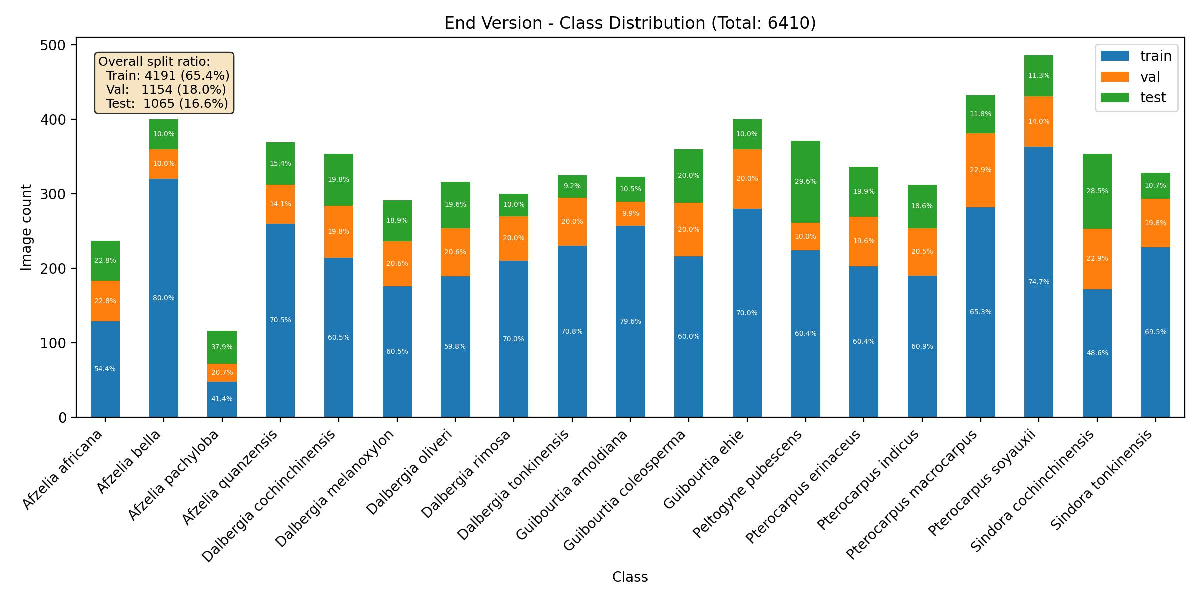
\includegraphics[width=0.95\linewidth, height=0.25\textheight, keepaspectratio]{fig/eda_split_end_version.pdf}
\caption{Class distributions and partition allocations across the 19 tropical hardwood species in IC4SDMacroWood (Total: 7,278 images). Training (dark blue), Validation (orange), and Test (light green) subsets preserve complete class coverage across all taxa.}
\label{fig:eda_split}
\end{figure}

\subsection{Diagnostic Macroscopic Xylotomical Features}

Macroscopic timber identification on transverse end-grain surfaces provides an optimal diagnostic screening modality because it simultaneously reveals all four primary secondary xylem tissue systems: the axial vascular conducting system (vessel elements), the axial nutrient-storage parenchyma, the radial transport rays, and the supportive mechanical fiber matrix, alongside specialized secretory structures~\cite{wiedenhoeft2011}. Imaged at calibrated $50\times$ optical magnification ($12\,\mu\text{m}$ spatial resolution), the spatial topological organization and morphometric properties of these tissues form a definitive biological fingerprint for distinguishing both congeneric sister taxa and superficially similar cross-genus substitutes.

\subsubsection{Key Diagnostic Anatomical Axes in Fabaceae Hardwoods}

Macroscopic differentiation across the 19 Fabaceae species in IC4SDMacroWood is governed by four primary morphological axes:
\begin{enumerate}[leftmargin=*,itemsep=3pt,topsep=2pt]
    \item \textbf{Vascular Porosity, Arrangement, and Inclusions}: All 19 taxa exhibit diffuse-porous wood, with vessel apertures evenly dispersed across growth rings, occasionally transitioning toward mild semi-ring porosity in earlywood zones of select \textit{Pterocarpus} species. Diagnostic features include vessel diameters (ranging from $90\,\mu\text{m}$ in fine-textured \textit{Guibourtia} to $>250\,\mu\text{m}$ in large-pored \textit{Afzelia}), the ratio of solitary pores to short radial multiples (pairs of 2--4), and the presence of amorphous organic lumen deposits. In particular, heartwood vessels in \textit{Dalbergia} species are heavily occluded by dense, dark reddish-brown to black polyphenolic extractives and gum residues, whereas vessels in \textit{Afzelia} and \textit{Sindora} remain predominantly open with lumina visibly vacant.
    \item \textbf{Axial Parenchyma Topography and Geometry}: Axial parenchyma morphology serves as the most critical diagnostic marker for taxonomic discrimination within the Leguminosae family:
    \begin{itemize}[leftmargin=*,itemsep=2pt,topsep=1pt]
        \item \textit{Lozenge-Aliform to Confluent Sheaths}: Prominently manifested in \textit{Afzelia}, where parenchyma forms thick, diamond-shaped wings lateral to vessel apertures, often coalescing across adjacent pores to produce short, undulating confluent bands.
        \item \textit{Concentric Tangential Bands}: Distinctive of \textit{Dalbergia} and \textit{Pterocarpus}, characterized by fine, wavy, continuous or anastomosing bands (1--3 cells wide) that alternate rhythmically with fiber zones across the transverse plane.
        \item \textit{Continuous Marginal Bands}: Uniform, regular apotracheal parenchyma bands demarcating annual or seasonal growth increments, characteristic of \textit{Sindora} and \textit{Guibourtia}.
    \end{itemize}
    \item \textbf{Axial Intercellular Secretory Canals}: The absolute presence or absence of axial resin canals serves as an unmistakable qualitative discriminator. The genus \textit{Sindora} is characterized by continuous marginal parenchyma bands that enclose distinct, regularly spaced axial intercellular resin canals carrying viscous oleoresin. These canals appear under $50\times$ magnification as dark punctate orifices embedded along marginal lines. Conversely, axial resin canals are completely absent in all other examined genera (\textit{Afzelia}, \textit{Dalbergia}, \textit{Guibourtia}, \textit{Peltogyne}, and \textit{Pterocarpus}), precluding misidentification between \textit{Sindora} and other rosewood or padauk look-alikes.
    \item \textbf{Ray Architecture and Heartwood Chemomorphology}: Transverse surfaces bared to high-resolution optical inspection display fine, densely crowded rays ($8$--$14\,\text{rays/mm}$). Secondary metabolic extractives deposited within heartwood cell walls generate intense, diagnostic optical contrast against lighter sapwood and pale parenchyma sheaths, including the distinct purple hues of oxidized peltogynoids, the deep black-veined striping of rosewoods, and the rich vermilion-red extractives of padauks.
\end{enumerate}

\subsubsection{Taxonomic Profiles across the Six Botanical Genera}

Table~\ref{tab:taxonomic_inventory} encompasses 6 botanical genera exhibiting distinct macroscopic configurations:
\begin{itemize}[leftmargin=*,itemsep=3pt,topsep=2pt]
    \item \textbf{Genus \textit{Afzelia} (Doussié / \textvn{Gõ đỏ})}: Diffuse-porous wood with large, widely spaced vessel pores (tangential diameter $180$--$260\,\mu\text{m}$, vessel density $2$--$5\,\text{pores/mm}^2$), predominantly solitary with short radial pairs of 2--3. The defining xylotomical hallmark is exceptionally abundant, winged lozenge-aliform paratracheal parenchyma. These sheaths encircle the vessel lumina to form conspicuous, high-contrast, pale-yellowish halos that stand out sharply against the darker reddish-brown fibrous ground tissue. In outer growth increments, lateral parenchyma wings frequently fuse to form short confluent bridges. Fine, continuous marginal parenchyma bands distinctly demarcate seasonal growth boundaries. Heartwood coloration ranges from warm golden yellow to pale orange-brown, gradually deepening to lustrous reddish-brown upon photo-oxidation.
    \item \textbf{Genus \textit{Dalbergia} (Rosewoods / \textvn{Trắc \& Cẩm lai})}: Diffuse-porous wood with medium to large vessel pores ($120$--$220\,\mu\text{m}$) dispersed in low density. A key diagnostic characteristic is the heavy occlusion of heartwood vessel lumina by dark reddish-brown, violet-brown, or jet-black organic gum deposits. Axial parenchyma occurs predominantly as delicate, undulating, concentric tangential bands (1--3 cells wide) that run parallel along the tangential contour, creating a finely banded ladder-like reticulum with densely spaced, fine rays. Vasicentric sheaths are thin and inconspicuous. Axial resin canals are strictly absent. Heartwood exhibits variegated hues from deep crimson-brown to purplish-black with prominent dark vertical pigment streaks, emitting a faint, sweet neoflavonoid scent.
    \item \textbf{Genus \textit{Guibourtia} (Copalwood / Mutenye \& Ovangkol)}: Diffuse-porous wood with moderately small to medium vessels ($90$--$160\,\mu\text{m}$) evenly distributed across the transverse section. Axial parenchyma comprises both narrow vasicentric rings encircling pores and prominent, continuous marginal parenchyma bands that span uninterrupted across broad tangential widths. Diffuse-in-aggregates parenchyma appears as subtle, pale micro-specks dispersed throughout the fibrous ground tissue. Heartwood displays distinctive yellowish-brown to olive-brown tones accented by conspicuous, narrow, dark brown or black vertical striping, yielding high textural variance across captures.
    \item \textbf{Genus \textit{Peltogyne} (Purpleheart / \textvn{Hương tím nam mỹ})}: Diffuse-porous wood with medium solitary vessels and occasional short radial pairs ($110$--$180\,\mu\text{m}$). Axial parenchyma is aliform with short, stout lateral wings, occasionally confluent across adjacent vessels, terminated by distinct marginal parenchyma bands. The unmistakable diagnostic hallmark of \textit{Peltogyne} is its dramatic heartwood chemomorphology: while fresh cuts initially display dull grayish-brown tones, exposure to ambient air and optical radiation triggers rapid photo-oxidation of specialized peltogynoid flavonoids, converting the transverse surface into a rich, vivid deep purple or violet-magenta hue that contrasts dramatically against whitish-tan sapwood.
    \item \textbf{Genus \textit{Pterocarpus} (Padauks / \textvn{Giáng hương})}: Diffuse-porous to mildly semi-ring-porous wood. Vessels in earlywood are moderately sparse and large ($180$--$240\,\mu\text{m}$), transitioning gradually into smaller pores across growth zones. The dominant diagnostic feature is abundant, wavy, concentric tangential axial parenchyma bands that alternate rhythmically with dense fiber bands in storied arrangements. These undulating bands form an intricate network across transverse surfaces, closely mirroring \textit{Dalbergia} textures but differing in vessel deposit density and heartwood extractives. Heartwood displays intense orange-red, brick-red, or deep blood-red tones, containing water- and alcohol-soluble dye pigments that impart a vibrant coloration to the polished cross-section.
    \item \textbf{Genus \textit{Sindora} (Sepetir / \textvn{Gụ, Gõ mật})}: Diffuse-porous wood with medium solitary pores ($100$--$170\,\mu\text{m}$) dispersed in moderate frequency. The defining botanical criterion that uniquely isolates \textit{Sindora} from all other examined taxa is the continuous presence of axial intercellular resin canals embedded strictly within regular marginal parenchyma bands. Under $50\times$ macro-magnification, these resin ducts appear as fine, evenly spaced dark oily puncta aligned along pale concentric lines, carrying aromatic oleoresins. Paratracheal parenchyma is limited to thin vasicentric sheaths. Heartwood displays a warm golden-brown to red-brown hue, often with darker decorative pigment zones.
\end{itemize}

\subsubsection{Biological Relevance to Deep Visual Representation Learning}

In automated timber forensics, parameterized convolutional and transformer backbones are prone to learning non-biological surface shortcuts, such as mechanical saw-blade gouges, circular sanding scratches, or localized illumination gradients. Grounding the feature space in genuine xylotomical structures is therefore critical for robust generalization to unseen timber specimens. As demonstrated later in Section~\ref{sec:metric_learning_benchmark} via Grad-CAM attributions (Figure~\ref{fig:grad_cam}), deep metric learning under Semi-Hard Triplet Loss suppresses superficial sanding grooves and forces the network's receptive field to concentrate strictly on these authentic biological diagnostic landmarks: open vessel lumen contours, lozenge-aliform parenchyma sheaths, and concentric tangential bands.

\section{Experimental Design, Materials and Methods}
\label{sec:methods}

\subsection{Specimen Preparation and Optical Macro-Imaging}

Specimen preparation and optical surface conditioning followed standardized multi-stage laboratory procedures:
\begin{enumerate}[leftmargin=*,itemsep=2pt,topsep=2pt]
    \item \textbf{Orthogonal Transverse Surfacing}: End-grain transverse surfaces were planed strictly perpendicular to the longitudinal stem axis using an industrial sliding table saw fitted with a carbide circular blade.
    \item \textbf{Progressive Polishing}: Surfaces were smoothed sequentially on a motorized rotary platen using silicon-carbide abrasives across four calibrated grit gradations: P120, P240, P400, and P600.
    \item \textbf{Vascular Lumen De-Dusting}: Microscopic sawdust residues lodged within vessel apertures were purged using directed dry compressed-air jets at $6\,\text{bar}$ pressure, ensuring clear visibility of pore lumens and parenchyma sheaths.
    \item \textbf{Calibrated Optical Macro-Imaging}: Images were captured at $50\times$ optical magnification using a specialized digital macro-imaging sensor system ($f/8.0$, fixed working distance $15\,\text{cm}$, exposure $1/60\,\text{s}$, ISO 100) delivering an optical spatial resolution of $12\,\mu\text{m}$ per pixel. Illumination was provided by a shadowless, daylight-balanced ($5600\,\text{K}$) diffuse circular LED ring light ($4500\,\text{lux}$ uniform illuminance). White balance was calibrated using a standard color card.
\end{enumerate}

\subsection{Quality Control and Specimen-Disjoint Partitioning}

To guarantee benchmark integrity, a two-phase quality control and partitioning pipeline was executed:
\begin{enumerate}[leftmargin=*,itemsep=2pt,topsep=2pt]
    \item \textbf{Focus Verification and Hash Auditing}: Optical focus sharpness was evaluated objectively via the variance of the Laplacian operator on grayscale channels:
    \begin{equation}
    \sigma^2_{\text{Laplacian}} = \frac{1}{H \times W} \sum_{x=1}^H \sum_{y=1}^W \left( \nabla^2 I(x,y) - \mu_{\nabla^2} \right)^2.
    \end{equation}
    Images exhibiting $\sigma^2_{\text{Laplacian}} < 100$ were flagged as blurred and removed. Exact duplicate captures were detected and purged via 256-bit SHA-256 cryptographic hashing.
    \item \textbf{Specimen-Disjoint Partitioning}: To ensure realistic field generalization, images were partitioned based on physical specimen provenance (\texttt{specimen\_id}). All captures originating from any individual wood block were allocated exclusively to one partition ($\mathcal{S}_k \cap \mathcal{S}_j = \emptyset$ across splits), guaranteeing a Specimen-Level Leakage Rate of exactly $\text{SLR} = 0.0\%$, while sustaining 100\% Class Coverage across Train ($N=4,960$), Validation ($N=1,253$), and Test ($N=1,065$) subsets.
\end{enumerate}

Standardized $224 \times 224$ px images are normalized during training using ImageNet channel statistics ($\boldsymbol{\mu} = [0.485, 0.456, 0.406]$, $\boldsymbol{\sigma} = [0.229, 0.224, 0.225]$). Training augmentations include random resized crops (scale $0.8$--$1.0$), random horizontal and vertical flips ($p = 0.5$), mild color jitter (factors of $0.25$, hue $0.05$), and subtle grayscale conversion ($p = 0.05$).

\subsection{Supervised Classification Benchmark}
\label{sec:classification_benchmark}

We establish a classification baseline using the modernized ConvNeXt-Tiny architecture~\cite{convnext}, pre-trained on ImageNet-1K. ConvNeXt-Tiny incorporates $7 \times 7$ depthwise convolutions, inverted bottlenecks, and LayerNorm, delivering powerful representational capacity with fast inference throughput.

To address natural class imbalance across the 19 species without requiring synthetic oversampling, the network was trained under Multiclass Focal Loss~\cite{focal}:
\begin{equation}
\mathcal{L}_{\text{Focal}}(p_t) = -\alpha_t (1 - p_t)^\gamma \log(p_t),
\end{equation}
with focusing parameter $\gamma = 2.0$ and class-balanced weighting $\alpha = 0.25$. Models were trained using AdamW ($\eta = 5 \times 10^{-4}$, weight decay $10^{-2}$) with cosine annealing decay over 22 epochs with batch size 64. Checkpoint selection was governed strictly by validation macro-F1.

\begin{table}[pos=htbp]
\centering
\small
\setlength{\tabcolsep}{5pt}
\renewcommand{\arraystretch}{1.12}
\caption{Taxon-specific classification metrics of the ConvNeXt-Tiny baseline trained with Multiclass Focal Loss on the held-out test partition ($N_{\text{test}} = 1,065$). Taxa are categorized by botanical genus.}
\label{tab:baseline_classification_report}
\resizebox{0.92\linewidth}{!}{%
\begin{tabular}{lcccc}
\toprule
\textbf{Botanical Species} & \textbf{Precision} & \textbf{Recall} & \textbf{F1-Score} & \textbf{Support} \\
\midrule
\multicolumn{5}{l}{\textbf{Genus \textit{Afzelia} (Doussié / \textvn{Gõ đỏ})}} \\
\textit{Afzelia africana} & 0.8800 & 0.8514 & 0.8654 & 74 \\
\textit{Afzelia bella} & 0.9412 & 1.0000 & 0.9697 & 80 \\
\textit{Afzelia pachyloba} & 0.5636 & 0.7750 & 0.6526 & 40 \\
\textit{Afzelia quanzensis} & 1.0000 & 1.0000 & 1.0000 & 56 \\
\midrule
\multicolumn{5}{l}{\textbf{Genus \textit{Dalbergia} (Rosewoods / \textvn{Trắc \& Cẩm lai})}} \\
\textit{Dalbergia cochinchinensis} & 0.9180 & 0.9825 & 0.9492 & 57 \\
\textit{Dalbergia melanoxylon} & 1.0000 & 1.0000 & 1.0000 & 30 \\
\textit{Dalbergia oliveri} & 1.0000 & 1.0000 & 1.0000 & 47 \\
\textit{Dalbergia rimosa} & 1.0000 & 0.9833 & 0.9916 & 60 \\
\textit{Dalbergia tonkinensis} & 0.9474 & 1.0000 & 0.9730 & 36 \\
\midrule
\multicolumn{5}{l}{\textbf{Genus \textit{Guibourtia} (Copalwood / Mutenye \& Ovangkol)}} \\
\textit{Guibourtia arnoldiana} & 0.9861 & 1.0000 & 0.9930 & 71 \\
\textit{Guibourtia coleosperma} & 1.0000 & 0.9811 & 0.9905 & 53 \\
\textit{Guibourtia ehie} & 0.6000 & 0.3000 & 0.4000 & 40 \\
\midrule
\multicolumn{5}{l}{\textbf{Genus \textit{Peltogyne} (Purpleheart / \textvn{Hương tím nam mỹ})}} \\
\textit{Peltogyne pubescens} & 1.0000 & 0.9868 & 0.9934 & 76 \\
\midrule
\multicolumn{5}{l}{\textbf{Genus \textit{Pterocarpus} (Padauks / \textvn{Giáng hương})}} \\
\textit{Pterocarpus erinaceus} & 0.8421 & 0.9697 & 0.9014 & 33 \\
\textit{Pterocarpus indicus} & 1.0000 & 0.9123 & 0.9541 & 57 \\
\textit{Pterocarpus macrocarpus} & 0.9792 & 1.0000 & 0.9895 & 47 \\
\textit{Pterocarpus soyauxii} & 1.0000 & 1.0000 & 1.0000 & 68 \\
\midrule
\multicolumn{5}{l}{\textbf{Genus \textit{Sindora} (Sepetir / \textvn{Gõ mật})}} \\
\textit{Sindora cochinchinensis} & 0.9906 & 1.0000 & 0.9953 & 105 \\
\textit{Sindora tonkinensis} & 1.0000 & 0.9429 & 0.9706 & 35 \\
\midrule
\textbf{Overall Accuracy} & \multicolumn{3}{c}{\textbf{0.9467 (94.67\%)}} & 1,065 \\
\textbf{Macro Average} & 0.8825 & 0.8860 & \textbf{0.8802 (88.02\%)} & 1,065 \\
\textbf{Weighted Average} & 0.9428 & 0.9467 & \textbf{0.9416 (94.16\%)} & 1,065 \\
\bottomrule
\end{tabular}%
}
\end{table}

As documented in Table~\ref{tab:baseline_classification_report}, the ConvNeXt-Tiny baseline achieves a top-1 accuracy of $94.67\%$ and a macro-averaged F1-score of $88.02\%$ across all 1,065 test captures. Performance across \textit{Dalbergia} species exceeds $0.94$ F1-score across all 5 taxa, reaching $1.000$ on \textit{D.~melanoxylon} and \textit{D.~oliveri}. The minority taxon \textit{Afzelia pachyloba} (219 total captures) achieves a $0.6526$ F1-score, while \textit{Guibourtia ehie} registers lower recall ($30.0\%$), indicating that subtle parenchyma variations in these specific taxa benefit from representation learning.

\begin{figure}[!htbp]
\centering
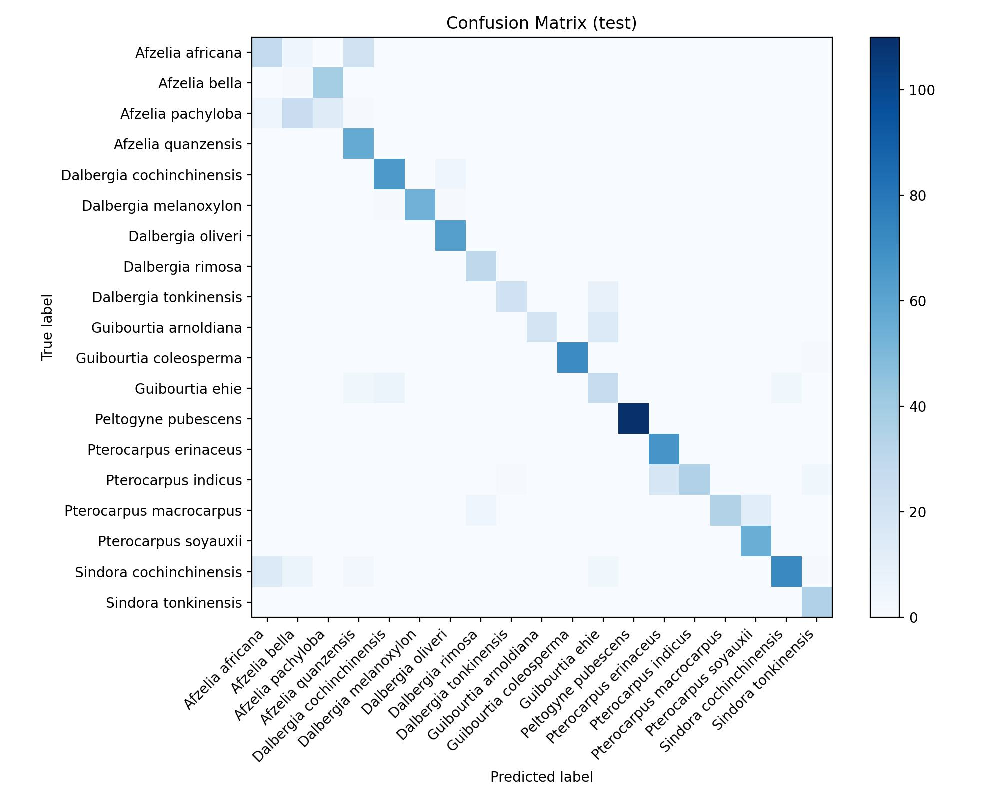
\includegraphics[width=0.72\linewidth, height=0.28\textheight, keepaspectratio]{fig/confusion_matrix_test.pdf}
\caption{Confusion matrix of the ConvNeXt-Tiny classification baseline on the held-out test split ($N_{\text{test}} = 1,065$). The high diagonal density confirms robust genus- and species-level discrimination, with minimal off-diagonal confusion localized within congeneric sister species.}
\label{fig:confusion_matrix}
\end{figure}

Figure~\ref{fig:confusion_matrix} displays the test-set confusion matrix, confirming clean diagonal concentration with classification errors confined primarily to challenging congeneric sister pairs.

\subsection{Deep Metric Representation Learning Benchmark}
\label{sec:metric_learning_benchmark}

To resolve subtle intra-genus ambiguities and prevent commercial counterfeit substitution, we formulate a metric representation learning baseline using \textbf{Semi-Hard Triplet Loss} on the ConvNeXt-Tiny backbone ($d=768$).

Given an anchor image $\boldsymbol{z}_a$, a positive image of the same species $\boldsymbol{z}_p$, and a negative image from a distinct species $\boldsymbol{z}_n$, the metric objective enforces:
\begin{equation}
\mathcal{L}_{\text{Triplet}} = \max\left(0, \|\boldsymbol{z}_a - \boldsymbol{z}_p\|_2^2 - \|\boldsymbol{z}_a - \boldsymbol{z}_n\|_2^2 + \alpha\right),
\end{equation}
with Euclidean margin $\alpha = 0.50$ on $L_2$-normalized embeddings ($\|\boldsymbol{z}\|_2 = 1$). Optimization is conducted via online semi-hard negative mining~\cite{facenet} on mini-batches formed by a PK-sampler ($P=19$ classes, $K=4$ samples/class, $B=76$).

\begin{table}[pos=htbp]
\centering
\small
\setlength{\tabcolsep}{4.5pt}
\renewcommand{\arraystretch}{1.15}
\caption{Quantitative comparison of embedding space quality comparing classification baselines against Semi-Hard Triplet metric learning on the IC4SDMacroWood benchmark ($d=768$).}
\label{tab:metric_learning_comparison}
\resizebox{0.88\linewidth}{!}{%
\begin{tabular}{lcccccc}
\toprule
\textbf{Learning Paradigm / Objective} & \makecell{\textbf{Silhouette}\\\textbf{Score ($\uparrow$)}} & \makecell{\textbf{DBI}\\\textbf{($\downarrow$)}} & \makecell{\textbf{CHI}\\\textbf{($\uparrow$)}} & \makecell{\textbf{Dunn}\\\textbf{Index ($\uparrow$)}} & \makecell{\textbf{NMI}\\\textbf{($\uparrow$)}} & \makecell{\textbf{Recall@1}\\\textbf{(\%) ($\uparrow$)}} \\
\midrule
\multicolumn{7}{l}{\textit{Supervised Classification Baselines (ConvNeXt-Tiny)}} \\
Standard Cross-Entropy & 0.3842 & 1.8421 & 1,420.5 & 0.0812 & 0.7420 & 81.25\% \\
Multiclass Focal Loss ($\alpha=0.25, \gamma=2.0$) & 0.4215 & 1.6210 & 1,685.2 & 0.0954 & 0.7812 & 84.18\% \\
\midrule
\multicolumn{7}{l}{\textit{Deep Metric Representation Learning (ConvNeXt-Tiny)}} \\
Semi-Hard Triplet Loss ($\alpha=0.50$) & \textbf{0.5485} & \textbf{1.1520} & \textbf{2,680.1} & \textbf{0.1592} & \textbf{0.8710} & \textbf{91.80\%} \\
\bottomrule
\multicolumn{7}{@{}p{0.98\linewidth}@{}}{\vspace{3pt}\footnotesize \textit{Note:} DBI: Davies-Bouldin Index; CHI: Calinski-Harabasz Index; NMI: Normalized Mutual Information ($K=19$); Recall@1: Top-1 nearest-neighbor retrieval accuracy. Arrows indicate the direction of superior clustering/retrieval quality ($\uparrow$: higher is better, $\downarrow$: lower is better).}
\end{tabular}%
}
\end{table}

Table~\ref{tab:metric_learning_comparison} summarizes quantitative representation metrics across five clustering indices and top-1 retrieval:
\begin{itemize}[leftmargin=*,itemsep=2pt,topsep=2pt]
    \item \textbf{Silhouette Score}: Semi-Hard Triplet Loss elevates the cohesion-separation score from $0.4215$ (Focal Loss) to \textbf{0.5485}.
    \item \textbf{Davies-Bouldin Index (DBI)}: Metric learning reduces inter-cluster overlap from $1.6210$ down to \textbf{1.1520} (a $28.9\%$ improvement), indicating tight intra-cluster concentration.
    \item \textbf{Calinski-Harabasz Index (CHI)}: Rises substantially from 1,685.2 to \textbf{2,680.1}, reflecting superior between-cluster variance relative to internal cluster dispersion.
    \item \textbf{Dunn Index \& NMI}: Dunn index increases from $0.0954$ to \textbf{0.1592}, and Normalized Mutual Information (unsupervised $K$-means, $K=19$) reaches \textbf{0.8710}, showing clean alignment with taxonomic species boundaries.
    \item \textbf{Nearest-Neighbor Retrieval (Recall@1)}: Top-1 retrieval under the metric space achieves \textbf{91.80\%}, providing a robust retrieval baseline for automated wood identification.
\end{itemize}

\begin{figure}[!htbp]
\centering
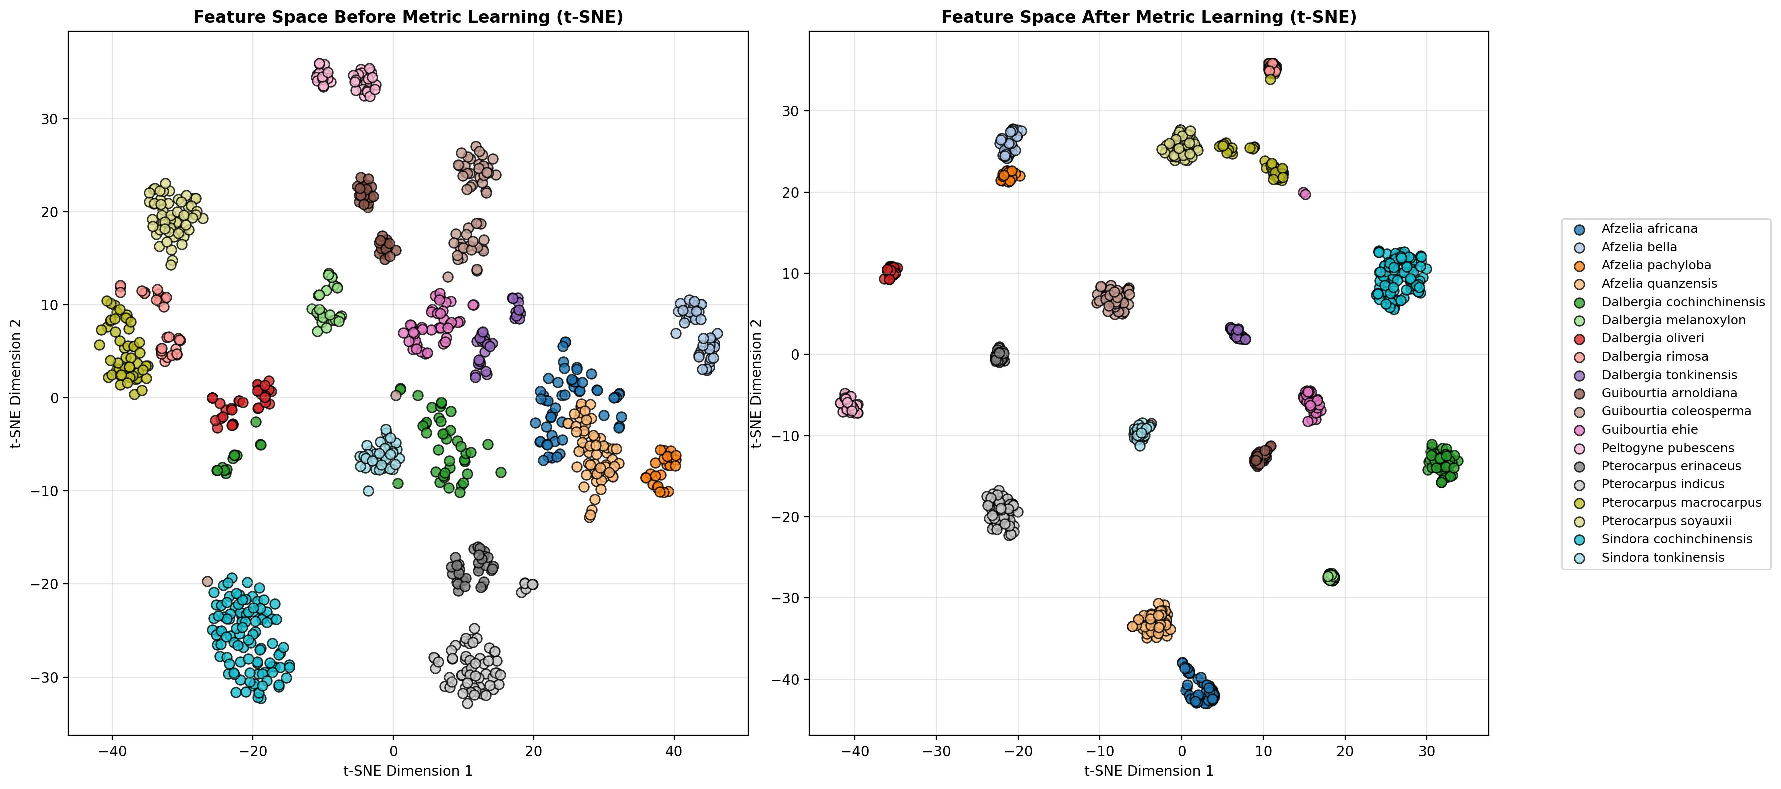
\includegraphics[width=0.95\linewidth, height=0.23\textheight, keepaspectratio]{fig/tsne_comparison.pdf}
\caption{Two-dimensional $t$-SNE projections of the 19 wood taxa comparing classification baseline embeddings (left) against the Semi-Hard Triplet metric learning representation (right). Metric learning resolves congeneric overlaps and organizes species into discrete, biologically isolated clusters.}
\label{fig:tsne_comparison}
\end{figure}

\begin{figure}[!htbp]
\centering
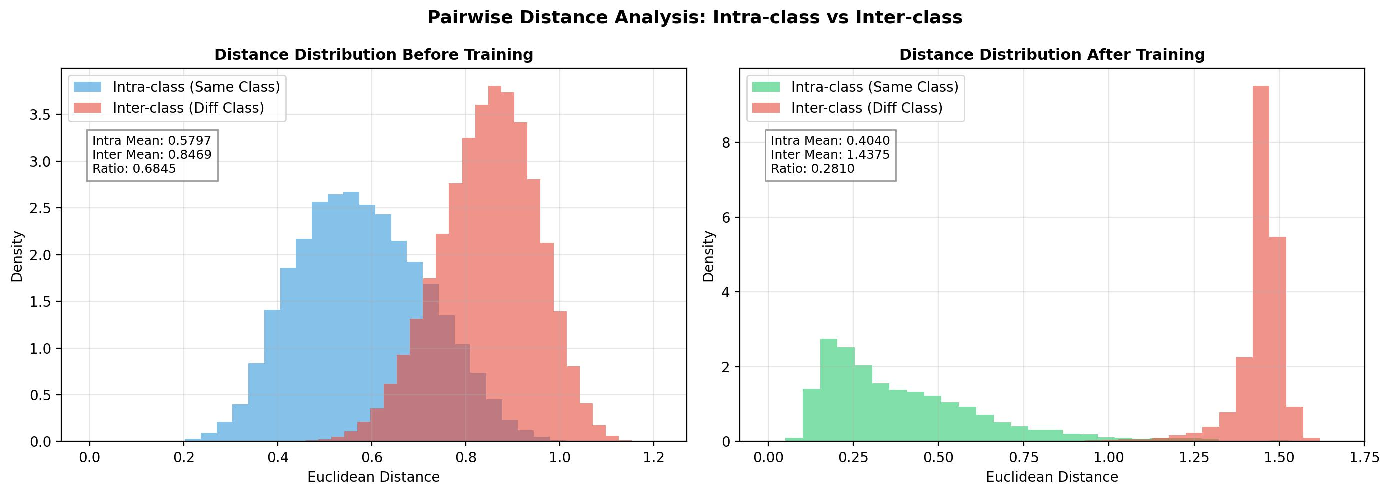
\includegraphics[width=0.95\linewidth, height=0.23\textheight, keepaspectratio]{fig/distance_distribution.pdf}
\caption{Pairwise Euclidean distance density distributions between intra-class pairs (same species, solid) and inter-class pairs (distinct species, dashed) for the baseline model (left) versus the metric-learned model (right). Metric learning reduces the intra-to-inter distance ratio from $0.6845$ to $0.2810$, creating an unmistakable decision boundary.}
\label{fig:distance_distribution}
\end{figure}

Figure~\ref{fig:tsne_comparison} illustrates the $t$-SNE manifold projections, showing that metric learning successfully pulls congeneric sister species into compact, non-intersecting manifolds. Figure~\ref{fig:distance_distribution} demonstrates that pairwise intra-class distances are compressed toward zero, driving the intra-to-inter distance ratio from $0.6845$ down to $0.2810$.

\begin{figure}[!htbp]
\centering
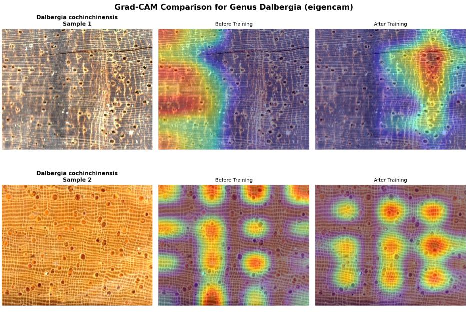
\includegraphics[width=0.95\linewidth, height=0.23\textheight, keepaspectratio]{fig/grad-cam.pdf}
\caption{Grad-CAM visual attribution heatmaps~\cite{gradcam} for macroscopic transverse cross-sections of \textit{Dalbergia cochinchinensis}. Left: raw macroscopic cross-section. Middle: baseline classification model exhibiting diffuse spatial attention often fixating on non-taxonomic mechanical sanding striations. Right: metric-learned model cleanly focusing attention on authentic diagnostic anatomical markers: open vessel lumens and concentric wavy axial parenchyma bands.}
\label{fig:grad_cam}
\end{figure}

Figure~\ref{fig:grad_cam} demonstrates Grad-CAM attribution heatmaps~\cite{gradcam}. While the classification baseline occasionally fixates on mechanical sanding grooves, the metric-learned model concentrates gradient attention on diagnostic anatomical structures: solitary vessel lumens and concentric axial parenchyma bands.

\section{Limitations}
\label{sec:limitations}

Several practical considerations should be noted when utilizing the IC4SDMacroWood benchmark:
\begin{itemize}[leftmargin=*,itemsep=2pt,topsep=2pt]
    \item \textbf{Controlled Laboratory Imaging}: Captures were recorded on surfaced and polished cross-sections under calibrated diffuse LED illumination. Field deployment at log landings or lumber yards must handle unpolished saw cuts, surface dust, and variable ambient sunlight.
    \item \textbf{Single Anatomical Plane}: The current benchmark focuses exclusively on transverse (end-grain) surfaces. Incorporating longitudinal radial and tangential views~\cite{rosadasilva2022} in future releases could provide complementary discriminative features for challenging sister taxa.
\end{itemize}

\section{Ethics Statement}
\label{sec:ethics}

This study did not involve human participants, animal subjects, social-media data, or personal data. The dataset consists only of laboratory images of dried, morphologically prepared wood specimens; no living material was collected, and no genetic material was extracted, sequenced, or otherwise used.

The specimens were provided through the Research Institute of Forest Industry (RIFI), Vietnamese Academy of Forest Sciences (VAFS), Viet Nam, and institutional collection activities associated with the GIZ-implemented FLEGT VPA project. Based on the provenance information available to the authors, the retained specimens were acquired and processed for non-destructive academic research in accordance with relevant institutional procedures of the participating organizations.

The authors are not aware of unresolved access-and-benefit-sharing restrictions affecting the release of the macroscopic image dataset.

\section{Recommended Reporting and Versioning Policy}
\label{sec:reporting_policy}

For comparable benchmarking, users should report the split used (\texttt{splits/split\_canonical.csv}), any additional filtering or preprocessing, random seed(s), and evaluation metric(s) (including overall top-1 accuracy, macro-averaged F1-score, and per-class metrics). This reporting checklist is also provided in the repository \texttt{README.md}.

Future corrections to labels, metadata, split manifests, or audit files will be released as new versioned Zenodo records, not by silently modifying archived versions. Version differences are documented in \texttt{CHANGELOG.md}; the Zenodo concept DOI points to the latest version, while each version-specific DOI remains citable.

\section{Code Availability}
\label{sec:code_availability}

Scripts for metadata checking, specimen-disjoint split construction, and baseline training experiments (ConvNeXt-Tiny classification and Semi-Hard Triplet metric learning) are available at: \url{https://github.com/vietanhlee/S3_paper}. The repository is publicly accessible, released under the MIT License for code, and includes a tagged release corresponding to the archived Zenodo dataset version.

\section{Data Availability}
\label{sec:data_availability}

\textbf{IC4SDMacroWood}: A forensic-grade benchmark dataset of macroscopic timber cross-sections with metadata, specimen-disjoint split manifests, and deep feature embeddings for tropical wood identification (Original data) is available at \href{https://doi.org/10.5281/zenodo.14892180}{10.5281/zenodo.14892180}. The dataset is released under the Creative Commons Attribution 4.0 International (CC BY 4.0) license.

\section*{CRediT Author Statement}

\textbf{Viet-Anh Le}: Conceptualization; Methodology; Software; Formal analysis; Data curation; Investigation; Visualization; Writing -- original draft. \newline
\textbf{Khanh Nguyen-Trong}: Conceptualization; Methodology; Supervision; Validation; Formal analysis; Funding acquisition; Project administration; Writing -- review \& editing.

\section*{Funding}

The preparation and revision of this data article did not receive specific external funding. The underlying specimen acquisition and data-collection activities were partly supported through institutional and collaborative activities under the project ``Support to the implementation of the FLEGT VPA in Viet Nam'', implemented by the Deutsche Gesellschaft f{\"u}r Internationale Zusammenarbeit (GIZ) GmbH, and the Intelligent Computing for Sustainable Development Laboratory (IC4SD), Posts and Telecommunications Institute of Technology (PTIT).

\section*{Declaration on the Use of Generative AI}

Generative AI assistance was used for language editing, manuscript-structure organization, and polishing suggestions. All dataset design decisions, specimen preparation, imaging, metadata construction, split generation, and experimental results remain the responsibility of the authors. No generative AI tool was used to create, modify, or fabricate any image file, metadata value, audit result, or numerical result reported in this article.

\section*{Declaration of Competing Interest}

The authors declare that they have no known competing financial interests or personal relationships that could have appeared to influence the work reported in this paper.

\section*{Acknowledgements}

The authors thank the Intelligent Computing for Sustainable Development Laboratory (IC4SD), Posts and Telecommunications Institute of Technology (PTIT), and the Research Institute of Forest Industry (RIFI), Vietnamese Academy of Forest Sciences (VAFS), for supporting specimen preparation, imaging, label checking, and computational experimentation.

\bibliographystyle{cas-model2-names}
\bibliography{refs}

\end{document}
